Software testing is an investigation conducted to provide stakeholders with information about the quality of the software product or service. It is very critical step in the process of software development. It plays especially a decisive role of the secure and successful blockchain application development. A single bug in a smart contract can open a security hole wide enough for someone to reach in and steal the entire contents of your digital asset.
\section{Testing Environment}
Corda uses industry-standard tools and running environment:
\begin{itemize}
	\item Oracle JDK 8 JVM - minimum supported version 8u171
	\item IntelliJ IDEA - supported versions 2017.x and 2018.x (with Kotlin plugin version 1.2.51)
	\item Git
	\item database h2
	\item OS: Windows 10 and IOS
	\item Memory: 3GB RAM
	\item CPU: Intel 2 cores.
	
\end{itemize}

\section{Functional Test}
In order to ensure the correctness and validation of our project, taking functional test turns out to be absolutely critical and necessary. Further more, this part will vastly assist readers better understand the process and mechanism. In this section, Unlike the usual software development documentary, only the core functions  and carefully selected test cases will be presented. 

\subsection{Function 1: Add Box}


\subsection{Function 2: Deposit}

\subsection{Function 3: Refuel Fee}

\subsection{Function 4: Pledge}


\section{Integration Test}
After the unity and functional tests, Integration Test cannot be omitted, since it ensures that the integrated modules/components work properly, and detect the interface error.

In order to complete the test, we divide the whole test as following steps which was illustrated in the Figure, 
\begin{figure}[H]% order of placement preference: here, top, bottom
	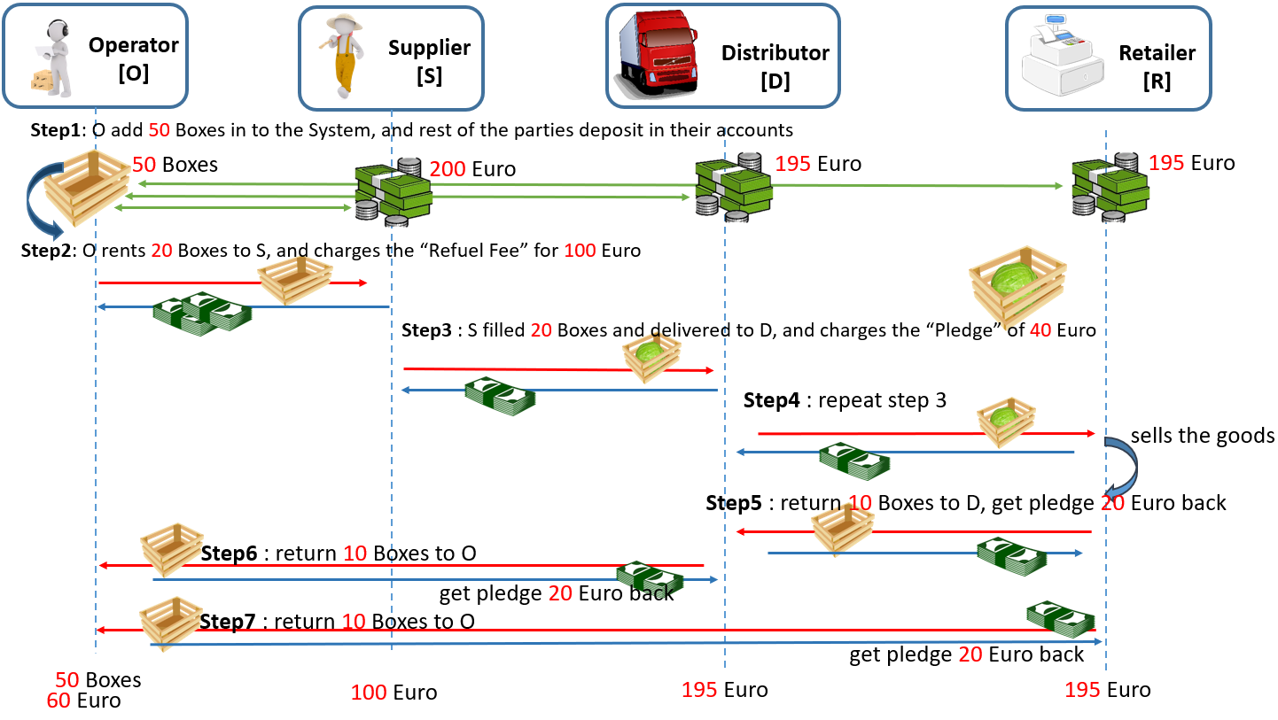
\includegraphics[width=\textwidth]{charts/c7-test-overview}
	\caption{The Cash and Box flow of PledgeContract}
\end{figure}



% ==================Performance=========================
\section{Performance Test}
Performance test plays a crucial role in our project. Whether leveraging the blockchain technology depends on how well and reliable it runs in reality. In this section, the expected features like high throughput, robustness, synchronization, etc are tested. 

However the Performance is multi-dimensional, multi-variable issue. In our cases, the performance highly relates to the following factors:
\begin{itemize}
	\item \textbf{Complexity of Contract and Flow.}\\
		The contracts and Flow contains the actual business logic, boundary conditions, and constraints. The more complicated they are, the slower performance would be. So it also provides us with the insight why and how we should optimize the program. Like in this project, the "Addbox" transaction in most cases is much faster than the "Refuel Fee" contract.
    \item \textbf{Consensus and Notary Type}\\
        The very classic argument is about the speed of "POW" and "POS", different consensus will vastly influence the performance. In Corda, it is via Contract's verification function and Notary' investigation to do the work.
        In our prototype, since the Corda blockchain doesn't have token, so the users have to transfer money offline; and because of no external reference, the Operator have to manually confirm the deposit from users.
    \item \textbf{Network and Infrastructure}\\
		This is quite important feature for any network-based application. For nodes running on local infrastructure, the number of cores, the CPU, the database.
\end{itemize}
\subsection{Throughput}
One of the core criteria when we estimate the system' performance. Taking the simplest transaction "AddBox" and the most complicated transaction "Pledge" as the test sample.

\subsection{Robustness and Recovery}
The stability and robustness of our system are estimated in the following perspectives.
\subsubsection{Node data storage}

\subsubsection{Recovery from node crashes}


\subsubsection{Recovery from corruption/deletion of the node's files}


\section{Features of this Project}
Though the previous steps have clearly demonstrated the functional features. However there are other characteristics of this Corda-based application, which need to be highlighted. It would be the very first-hand material and direct reference of people want to setup an analogous project. 

\subsubsection{Identifiable Participants and trustworthy counterparties}

\subsubsection{Multi-User and multiple permission}

\subsubsection{Pluggable Notary services}
 
\subsubsection{Multiple notaries}
 
\subsubsection{"Need-to-Know" mechanism}

\subsubsection{Confidentiality}

\section{Future work}

